\section{Executive Summary}
Stellen Sie sich eine voll belegte Werkstatt am Montagmorgen vor: Der Fehlerspeicher meldet „Dieselpartikelfilter: Differenzdruck zu hoch“, Hebebühnen sind knapp, der Kunde wartet. Was fehlt, ist nicht ein weiterer Code, sondern die wahre Ursache. Genau hier setzt \ac{KARL} Diagnostics an. Eine \ac{E2E}-Diagnoselösung aus robuster \ac{OBD}-II/\ac{CAN} Hardware (Kabel oder Funkadapter) und \ac{KI}-gestützter Cloud-Software. KARL fusioniert Fehlercodes, Live-Sensordaten, Herstellerdokumentation, Wissen aus Communities und externe Messgeräte zu präzisen, erklärbaren Reparaturempfehlungen inklusive priorisierter Hypothesen, Prüfschritte und Wahrscheinlichkeiten. Hinter einem „vollen“ Partikelfilter erkennt \ac{KARL} so etwa das defekte Thermostat als wahrscheinlichste Ursache, sichtbar in Temperatur- und Regenerationsmustern, auch ohne spezifischen Code.
\newline\newline
Für freie und markengebundene Werkstätten, Serviceketten, mobile Mechaniker, Flottenbetreiber und Prüfgesellschaften adressiert \ac{KARL} das Kernproblem steigender Komplexität bei Zeit- und Margendruck. Die Nutzen sind höhere \ac{FTFR}, weniger Teiletausch auf Verdacht, kürzere Standzeiten und produktive Unterstützung auch weniger erfahrener Mitarbeitender. Technisch setzt KARL auf eine hybride KI-Architektur aus regelbasierten Verfahren, neuronalen Netzen (z. B. LSTMs, Transformer) und einem Wissensgraphen. Jede Diagnose ist erklärbar; kontinuierliches Lernen aus realen, anonymisierten Werkstattfällen sowie Federated Learning verbessern die Performance fortlaufend, ohne Datenschutz zu gefährden. Im Wettbewerbsumfeld zwischen teuren, komplexen Premium-Testern (z. B. Bosch, Hella Gutmann), Nischenlösungen und \ac{OEM}-Tools positioniert sich KARL als herstellerunabhängige, kosteneffiziente und anwenderfreundliche Lösung mit \ac{KI}-gestützter Priorisierung, durchgängigen Prüfpfaden, \ac{OTA}-Updates und Integrationen in bestehende IT-Systeme.
\newline\newline
Der Markt wird getrieben von Elektrifizierung, softwaredefinierten Fahrzeugen und verschärften Vorgaben, somit steigt die Nachfrage nach \ac{SaaS}-Diagnose. \ac{KARL}s Go-to-Market startet mit Pilotierungen in DACH, Referenzkunden und Content-Marketing, gefolgt von schrittweiser Expansion in Europa. Vertrieblich kombinieren wir direkten \ac{B2B}-Verkauf mit Partnernetzwerken und technischen Kooperationen; integrationsseitig setzen wir auf Plug-and-Play in bestehenden Werkstattprozessen. Das Geschäftsmodell ist hybrid: einmalige Hardwareerlöse plus skalierbare Software-Abonnements pro Arbeitsplatz, ergänzt um Schulungen und Support. Kurzfristig investieren wir in Produktreife, Datenqualität, Zertifizierungen und Markteintritt; mittelfristig tragen Lizenzerlöse den größten Umsatzanteil bei bewusst margenträchtiger, aber nicht dominanter Hardware. Die Profitabilität ist nach ca. 2,5 Jahren geplant; zur Überbrückung negativer Cashflows sind Kredite von insgesamt rund 450.000 € vorgesehen.
\newline\newline
Hardware- und Software-\ac{MVP} bilden den Realisierungsplan, angfangen bei Auslieferung in kleinen Stückzahlen an Pilotkunden, schnelles Iterieren von Design, Funktionen und Produktionsprozessen, paralleler Aufbau der Fertigung und Akquise erster Kunden. Nach rund zwölf Monaten folgt der Markteintritt in Deutschland mit Fokus auf kleinere Werkstätten; anschließend breiteres Marketing, europäische Skalierung und perspektivisch eine selektive Öffnung Richtung \ac{B2C}. Chancen liegen in Netzwerkeffekten, Übertragbarkeit in angrenzende Domänen und dem wachsenden Bedarf an Diagnose-Know-how durch neue Antriebstechnologien. Risiken (Datenqualität, Zurückhaltung beim Wissensaustausch, rechtliche Fragen zur Datennutzung, \ac{OEM}-Wettbewerb, Investitionsbedarf) begegnen wir mit zusätzlichen Datenquellen, gezielten Roll-outs, Anreizsystemen, technischer Differenzierung und einer stringenten Partnerwahl. Operativ sichern agile Entwicklung, Qualitätsmanagement, Partnerintegration und internationale Skalierbarkeit die Umsetzung. Ein interdisziplinäres Kernteam aus Entwicklung, Data, Vertrieb und Einkauf gewährleistet schnelle Produktreife, Kundennähe und Lieferfähigkeit – flankiert von geplantem Teamausbau, Schulungen, Compliance-Prozessen und einer lernorientierten Kultur.

\section{Produkt \& Dienstleistung}
\label{sec:produkt}

\subsection{Problem \& Nutzenversprechen}
Moderne Fahrzeuge bringen eine hohe Systemkomplexität mit sich. Beispiele hierf"ur sind vernetzte Steuergeräte, eine Vielzahl an Sensoren sowie Hersteller- und modellabhängige Varianten. In der Werkstattpraxis führt dies zu Zeit- und Margendruck. Häufig werden Teile auf Verdacht getauscht, weil Fehlerspeicher nur Symptome melden, jedoch keine belastbaren Ursachen liefern. Die Folge sind niedrige Ersttrefferquoten, unnötige Fehlläufe und verlängerte Standzeiten. Gefordert ist eine Diagnose, die aus Symptomen verlässlich auf Ursachen schließt, Hypothesen transparent priorisiert und konkrete, effiziente Prüfschritte vorschlägt. Das Ergebnis sind höhere Ersttrefferquoten, kürzere Standzeiten und weniger Teiletausch auf Verdacht.

\emph{KARL Diagnostics}, das Künstliche-Auto-Reparatur-Lernsystem (KARL), verwandelt Fehlermeldungen und Livedaten in präzise Reparaturempfehlungen. Dazu kombiniert KARL robuste OBD/CAN-Diagnosehardware mit einer Cloud-Software, die Fehlercodes, Sensordatenströme, Expertenwissen und Foreninformationen zusammenführt. Das System liefert ursachenorientierte KI-Ergebnisse: priorisierte Hypothesen mit Wahrscheinlichkeiten, nachvollziehbare Prüfschritte und erklärende Begründungen, \emph{warum} ein Fehler auftritt, nicht nur \emph{dass} er auftritt. Jede bestätigte Reparatur fließt anonymisiert in die Modelle für alle Nutzer. 

Gegenüber klassischen Testern bietet KARL (i) ursachenorientierte \ac{KI} statt Code-Lesen, (ii) einen lernenden Algorithmus aus realen, anonymisierten Fällen und (iii) nahtlose Einbindung in bestehende Werkstattprozesse für \enquote{Plug-and-Play} in der Praxis. Die Hardware wird einmalig angeschafft; die Software wird pro Arbeitsplatz lizenziert. So bleiben die Einstiegshürden gering, der Nutzen skalierbar – und je mehr Datenpunkte einfließen, desto besser wird KARL.

\subsection{Produktübersicht: Hardware + Cloud-Software}
\ac{KARL} Diagnostics besteht aus mehreren eng verzahnten Bausteinen, die eine durchgängige Fehlerdiagnose vom Fahrzeug bis zur Cloud ermöglichen. Zum einen umfasst das System eine werkstatttaugliche OBD/CAN-Hardware für die Fahrzeuganbindung, zusätzliche Diagnosegeräte (Oszilloskop, Labornetzteil, Innenwiderstandsmesser, Multimeter) sowie eine leistungsfähige Cloud-Software. Diese Software verarbeitet eingehende Fehlercodes und Livedaten, leitet mittels künstlicher Intelligenz Ursachenhypothesen ab und ergänzt diese um strukturierte Prüfschritte mit zugehörigen Wahrscheinlichkeiten. Ziel ist ein \enquote{Plug-and-Play}-Einsatz in der Werkstatt bei maximaler Transparenz und Nachvollziehbarkeit der vorgeschlagenen Maßnahmen.

Die Fahrzeug-Schnittstelle ist robust, steckfertig und für den harten Dauerbetrieb in der Werkstatt konzipiert. Sie verfügt über ein stoßfestes Gehäuse, Öl- und Staubresistenz, eine kompakte Bauform sowie Status-LEDs für Verbindung und Logging. Zur Sicherstellung der Datenübertragung kommt ein redundantes System zum Einsatz, bestehend aus einer kabelgebundenen Schnittstelle und einer drahtlosen Anbindung via Bluetooth bzw. WLAN.
\begin{figure}[h!]
    \centering
    \begin{subfigure}[t]{0.45\linewidth}
        \centering
        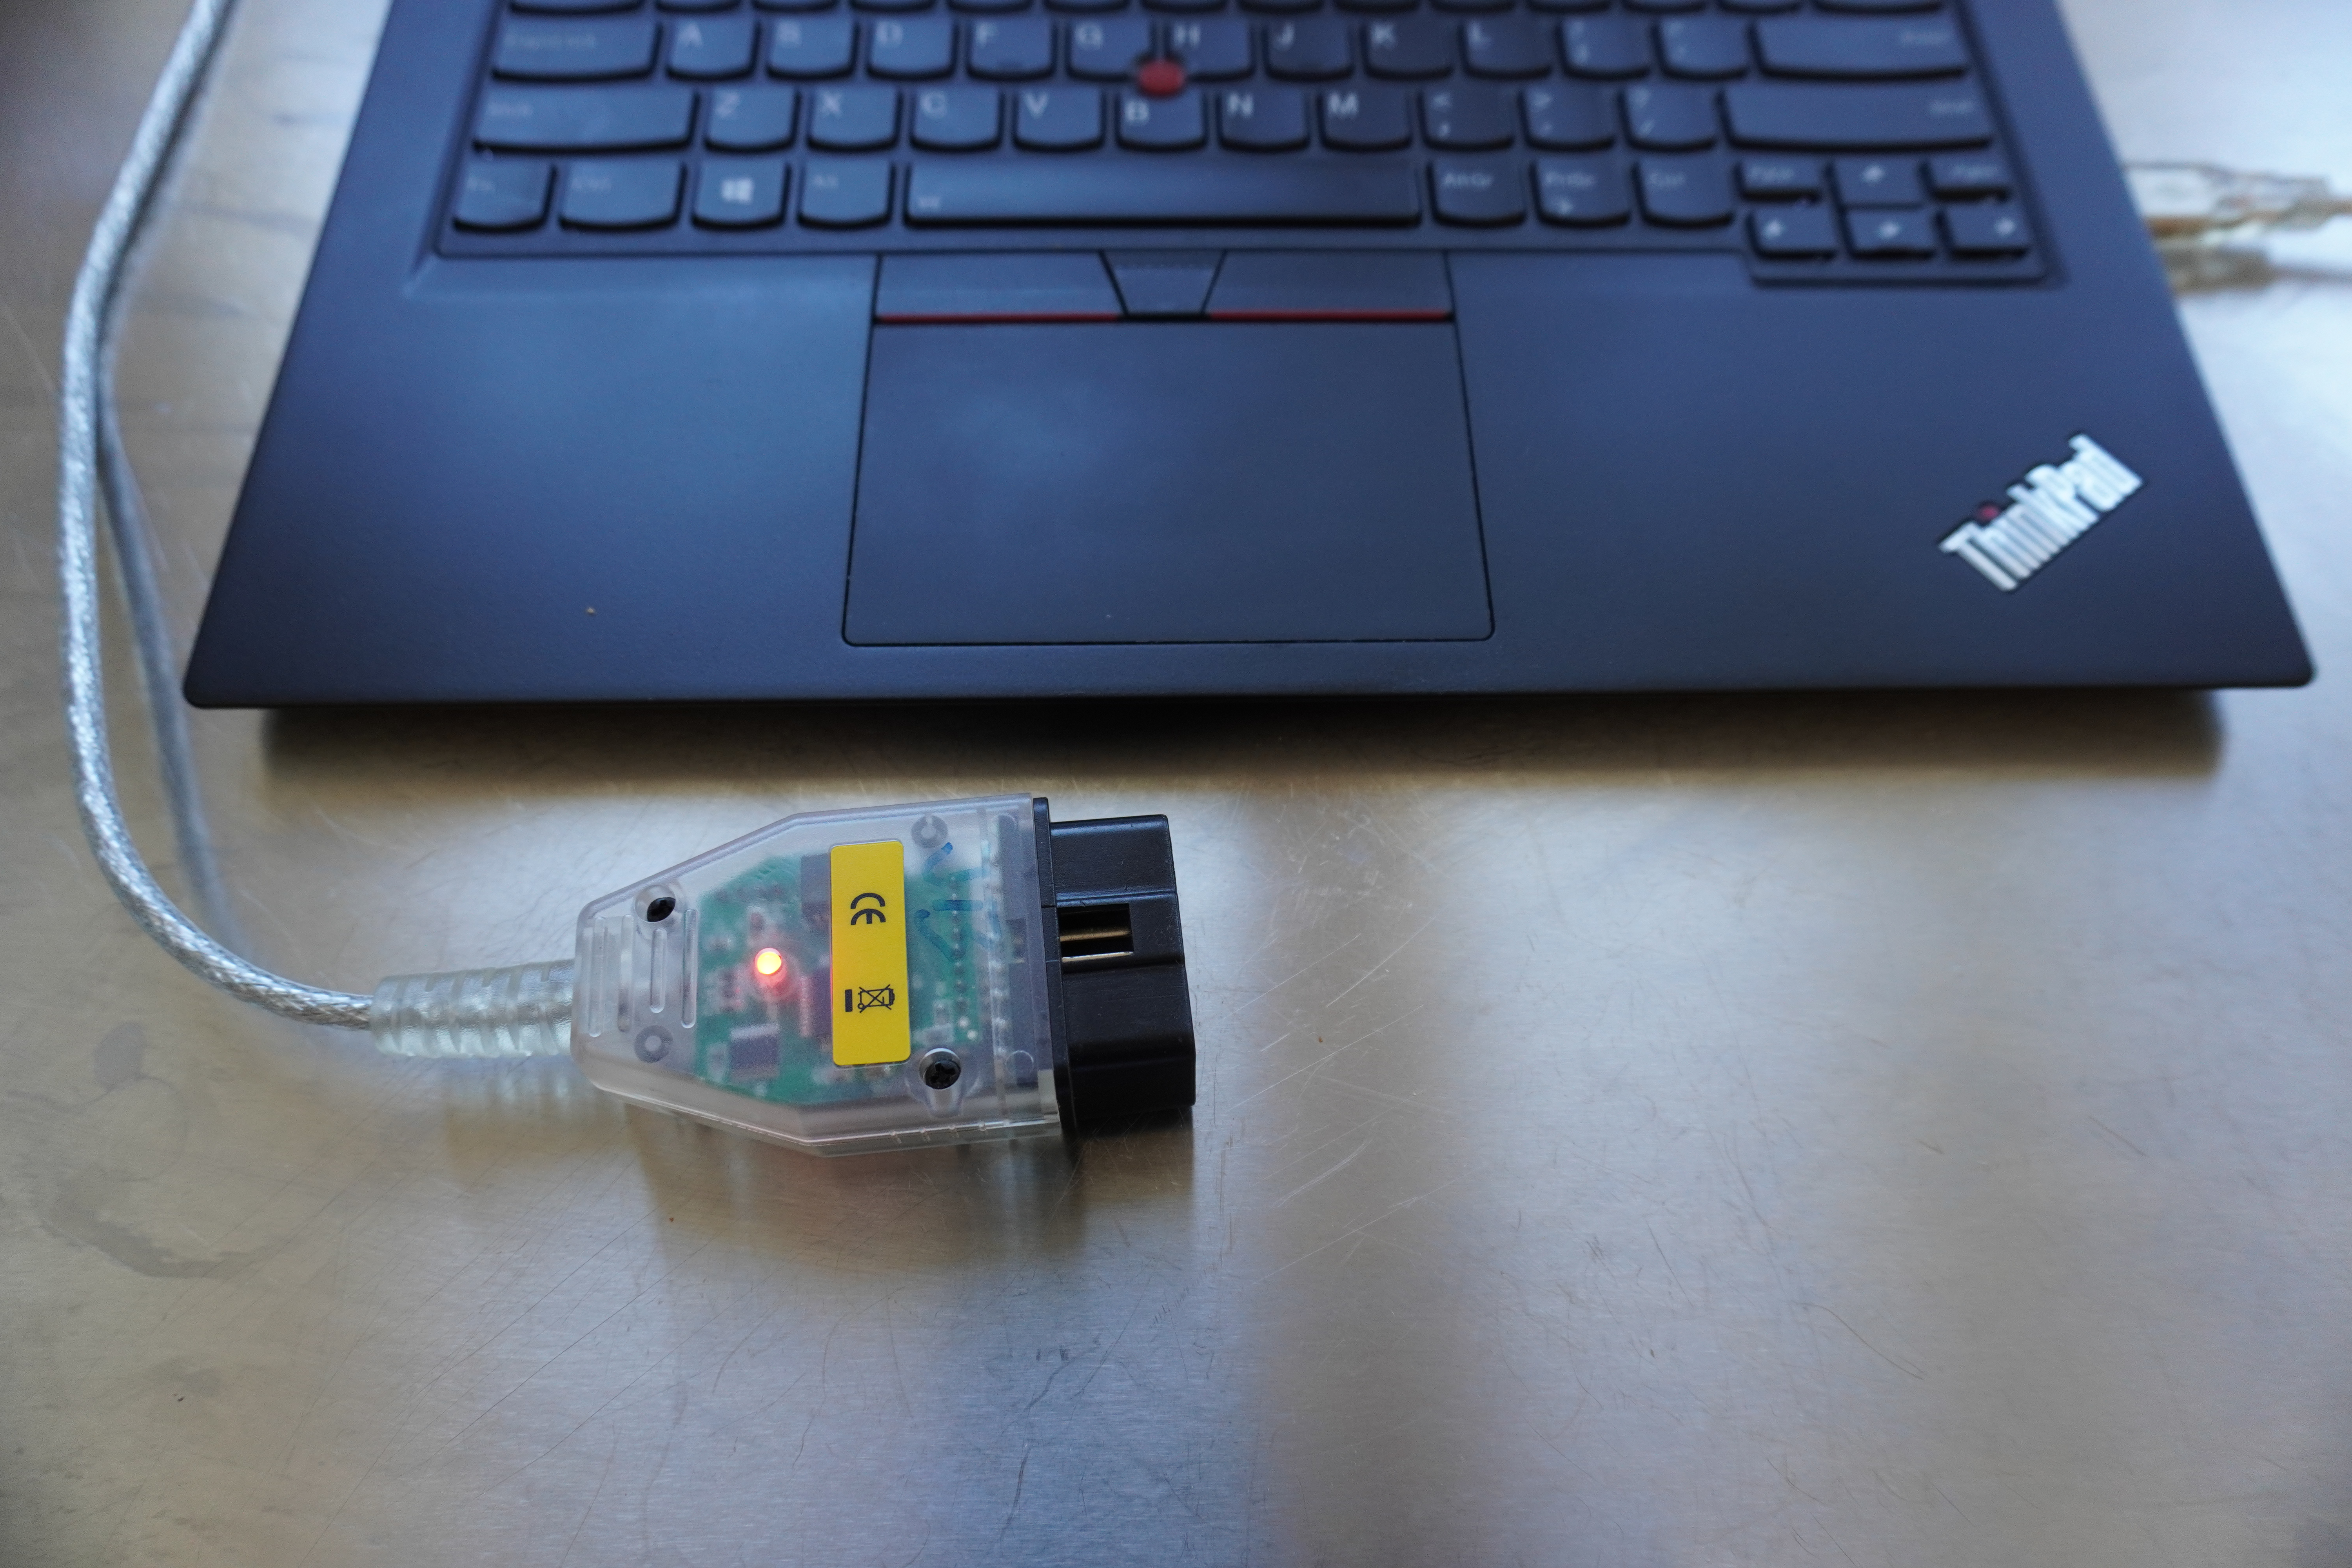
\includegraphics[width=\linewidth]{images/Hardware/obd_cable.JPG}
        \caption{OBD Kabel}
        \label{fig:obd_cable}
    \end{subfigure}
    \hfill
    \begin{subfigure}[t]{0.45\linewidth}
        \centering
        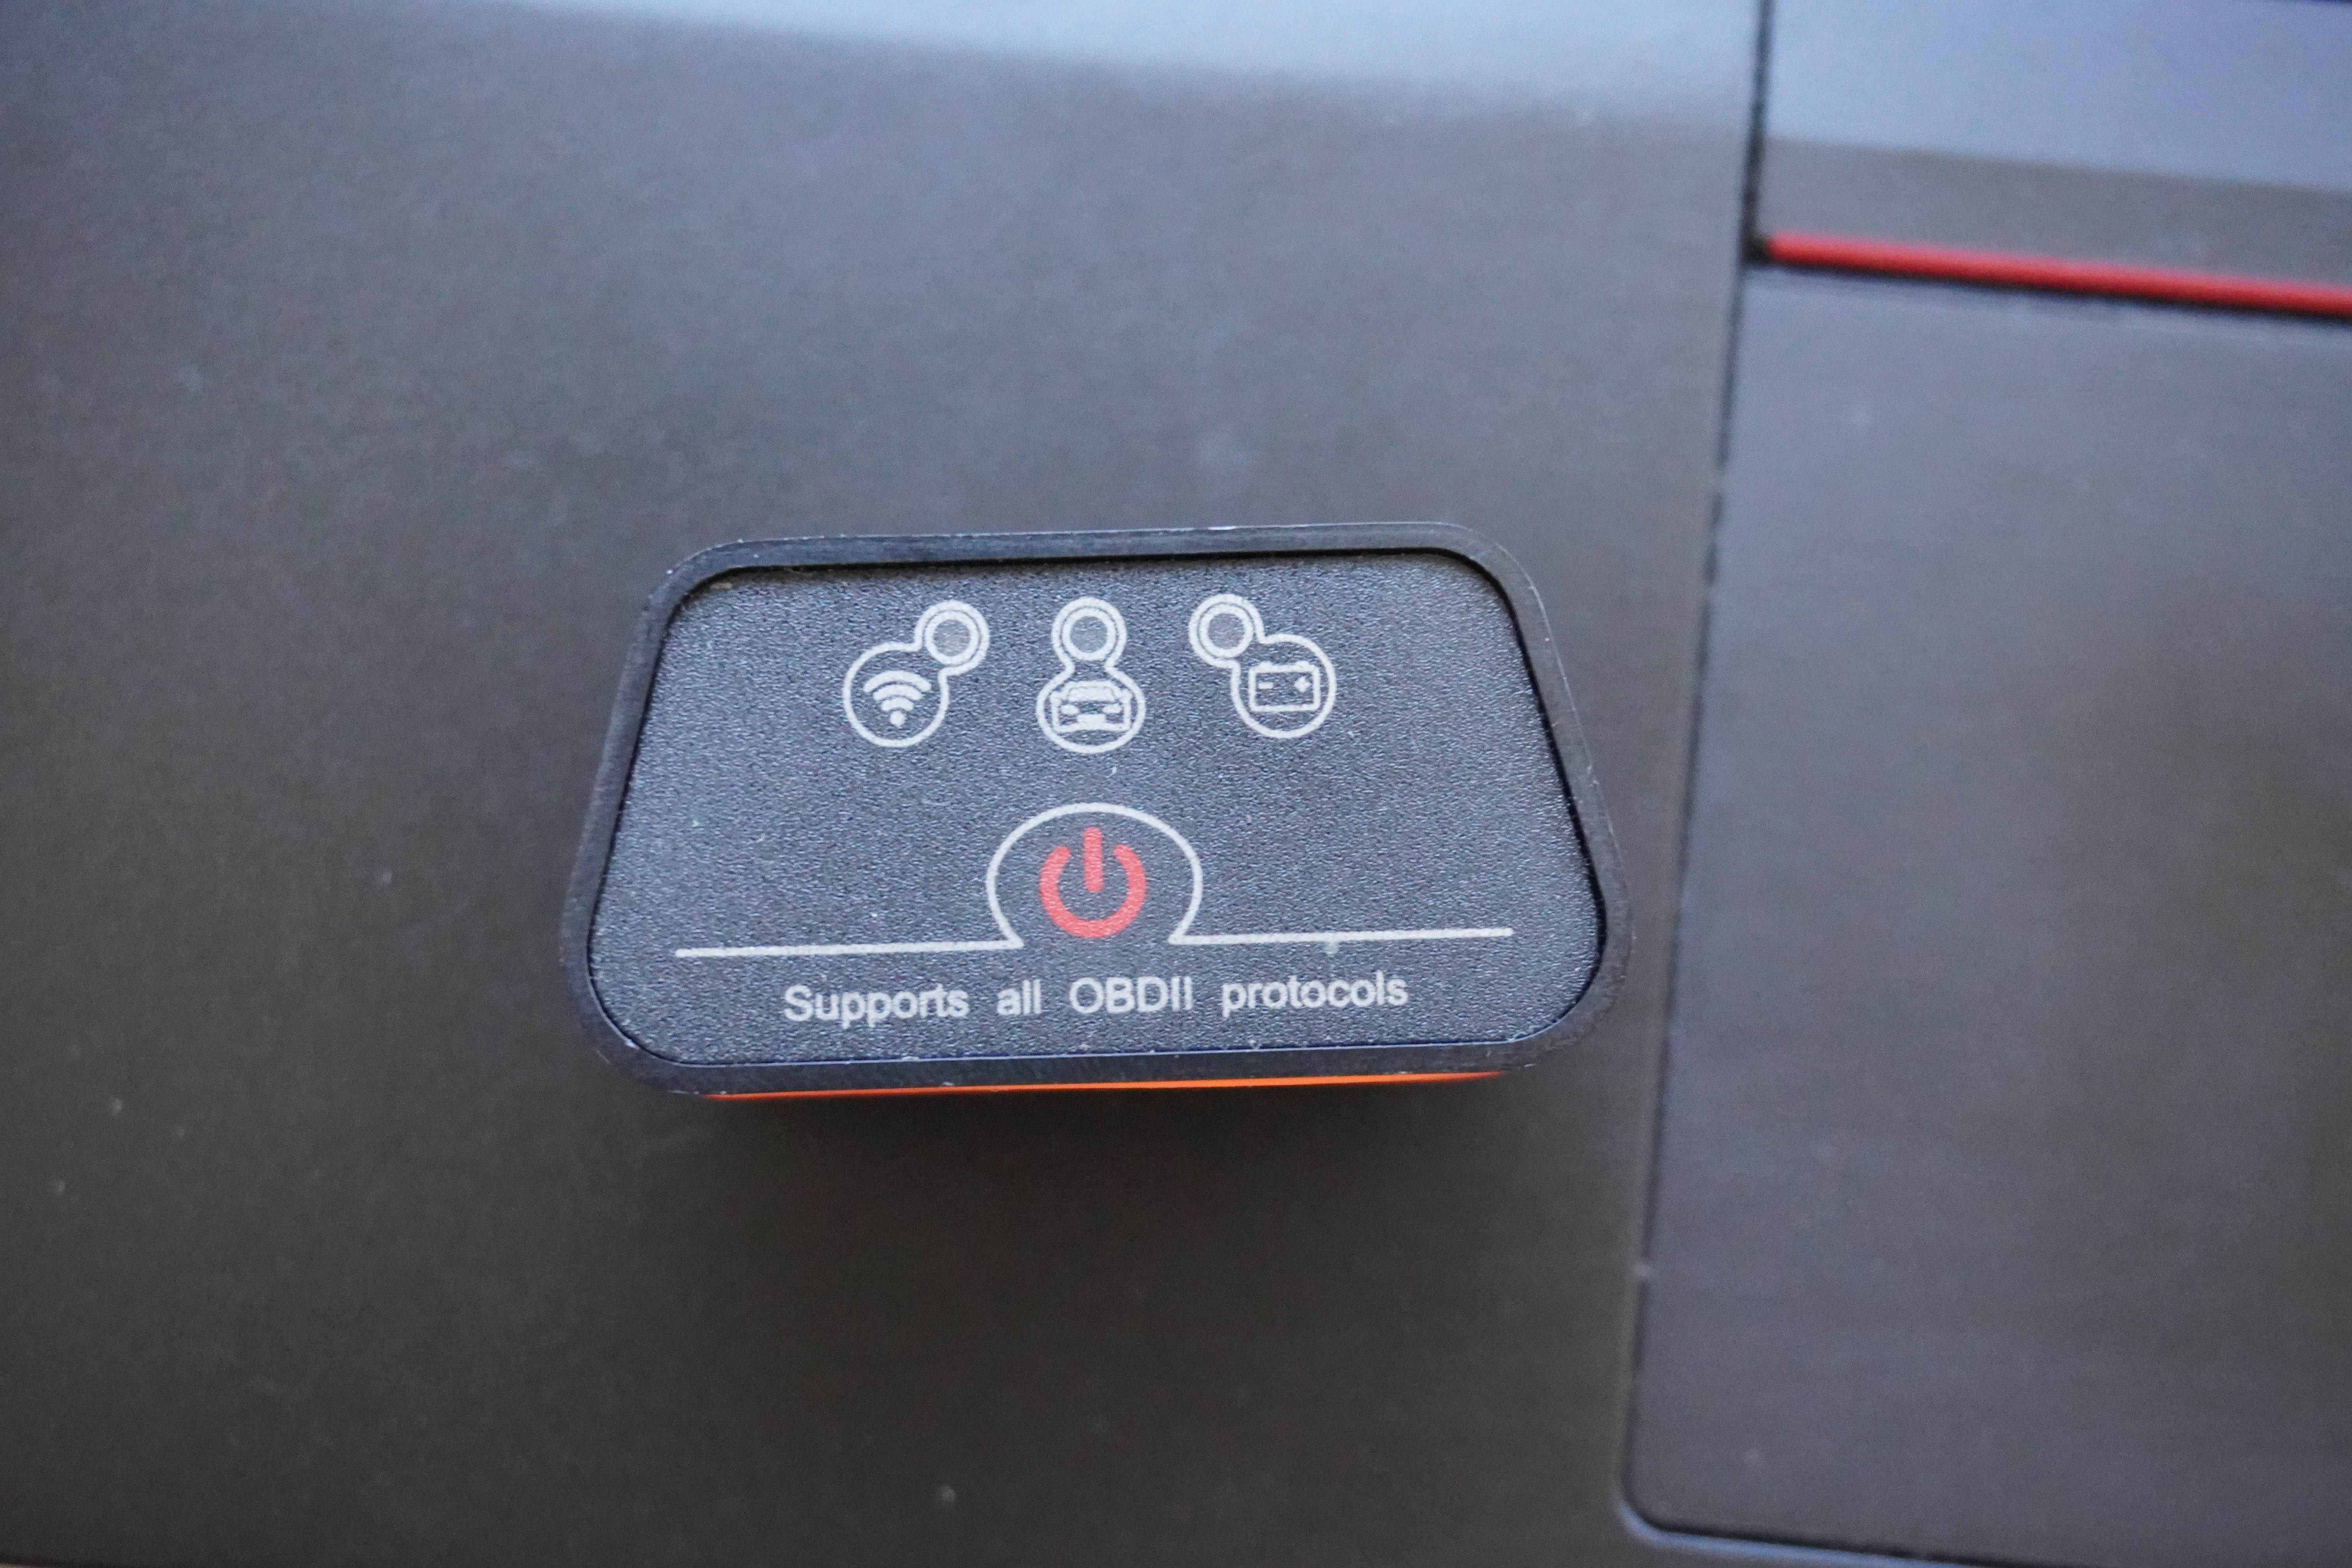
\includegraphics[width=\linewidth]{images/Hardware/obd_wifi.JPG}
        \caption{OBD WLAN-Adapter}
        \label{fig:obd_wifi}
    \end{subfigure}
    \caption{Vergleich von OBD Kabel und WLAN-Adapter}
    \label{fig:obd_comparison}
\end{figure}

Abbildung \ref{fig:obd_comparison} zeigt die beiden unterschiedlichen Systeme im Detail. Beim \ac{OBD}-II Kabel mit USB-Anschluss wird typischerweise ein Protokollcontroller wie der ELM327 oder der leistungsfähigere STN1110 eingesetzt. Diese unterstützen die gängigen \ac{OBD}-II Standards (CAN, ISO9141, KWP2000, J1850). Für die Anbindung an den PC wird zusätzlich ein USB-zu-Seriell-Wandler wie der FT232RL, CH340G oder CP2102 verwendet.  

In einem \ac{OBD}-II Bluetooth-/WLAN-Stick kommt im Kern ebenfalls ein ELM327- oder STN-Chip zum Einsatz. Dessen UART-Schnittstelle wird jedoch nicht mit USB, sondern mit einem Funkmodul verbunden, beispielsweise einem HC-05 oder RN-42 für Bluetooth Classic, einem HM-10 oder ESP32 für Bluetooth Low Energy oder einem ESP8266/ESP32 für WiFi. Beide Ansätze lassen sich somit kostengünstig mit handelsüblicher Hardware realisieren und bieten eine flexible Auswahl je nach Einsatzumgebung.

Zusätzlich kann die Diagnose durch externe Messgeräte wie Oszilloskop, Labornetzteil, Innenwiderstandsmesser oder Multimeter erweitert werden. Diese liefern wertvolle Messdaten, die über eine Sprachschnittstelle in den Diagnoseprozess einbezogen werden können. Auch wenn dieser Schritt optional ist, ermöglicht er eine noch genauere Eingrenzung und Bestätigung der Fehlerursachen.

Die Aggregation aller erfassten Informationen erfolgt in der Cloud. Dort analysieren KI-Modelle die Daten und geben konkrete Diagnoseempfehlungen mit Schritt-für-Schritt-Anleitungen aus. Das System greift dabei sowohl auf offizielle Herstellerdokumentationen als auch auf Erfahrungswissen aus Foren zurück. Gerade letzteres erweist sich als äußerst nützlich bei älteren Fahrzeugmodellen, für die Hersteller häufig nur unzureichende Informationen zu später auftretenden Problemen bereitstellen. Durch die Integration von Schwarmintelligenz aus Online-Communities können somit auch komplexe oder seltene Fehlerbilder zuverlässig erkannt werden.

\begin{figure}[h!]
    \centering
    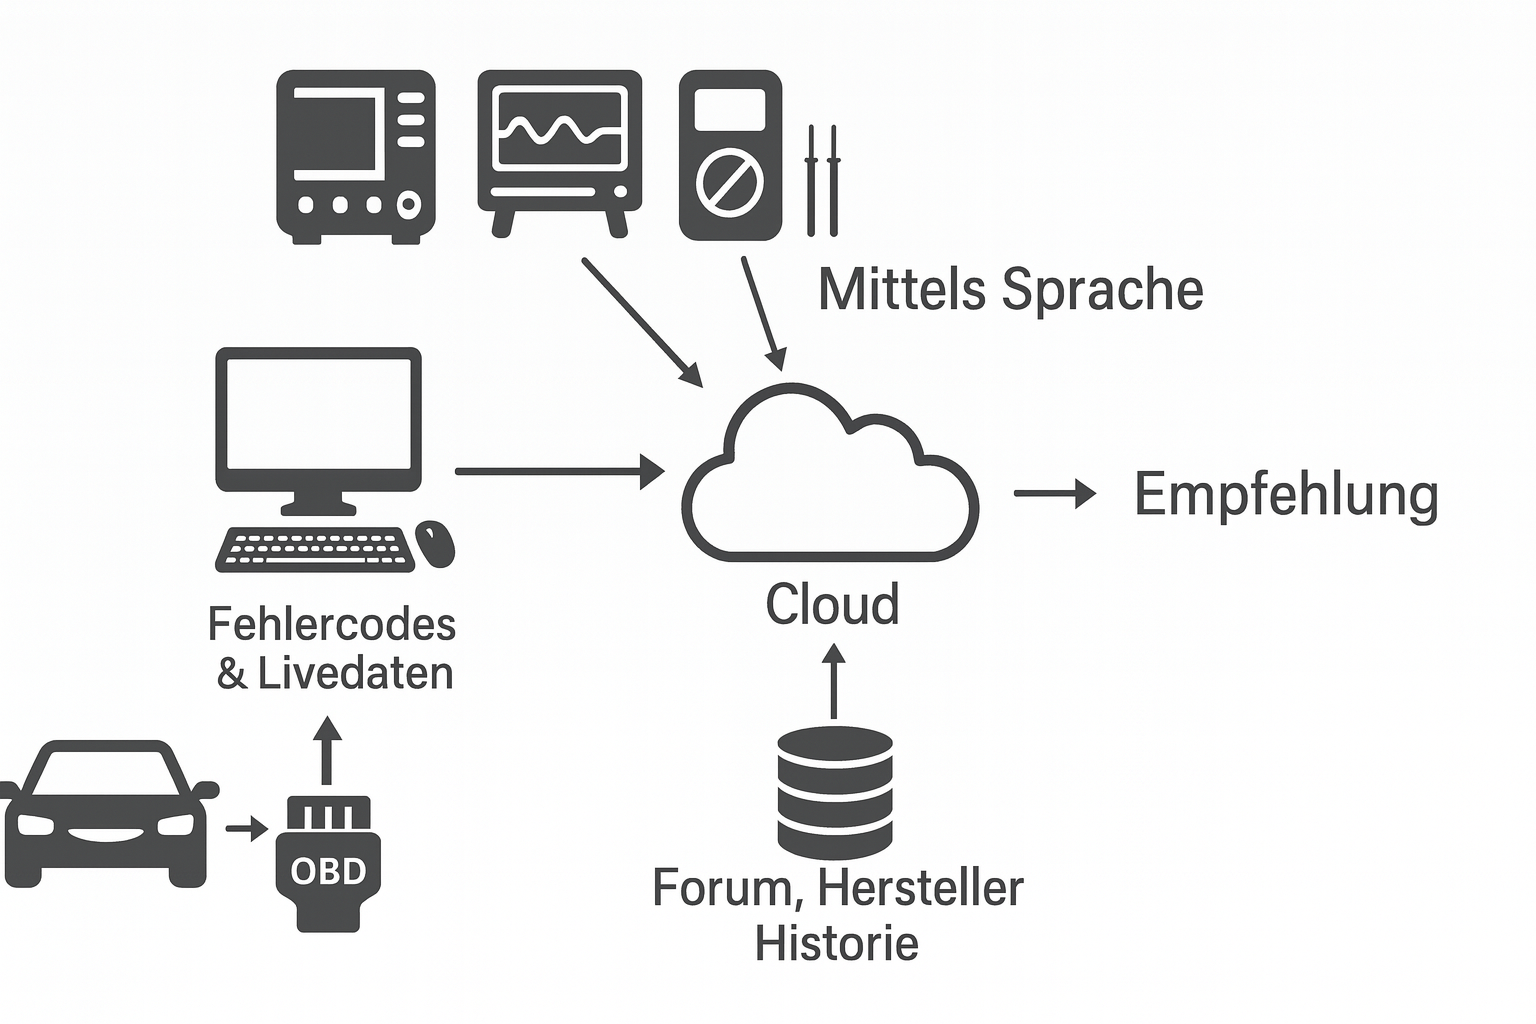
\includegraphics[width=1\linewidth]{images//Hardware/ChatGPT Image Aug 31, 2025, 04_03_25 PM.png}
    \caption{Systemarchitektur von KARL Diagnostics mit Fahrzeuganbindung, Zusatzhardware und Cloud-Komponenten}
    \label{fig:placeholder}
\end{figure}

Die Benutzeroberfläche des Diagnosesystems läuft unter Windows, sodass die Werkstatt jede handelsübliche PC-Hardware nutzen kann. Die Software wird lokal installiert und kommuniziert in Echtzeit mit der angeschlossenen Hardware sowie der Cloud.



Abbildung \ref{fig:placeholder} zeigt die Gesamtarchitektur des Systems sowie die wichtigsten Funktionsbausteine im Überblick.


\subsection{KI-Ansatz \& Erklärbarkeit}

Das \ac{KI}-System von \ac{KARL} Diagnostics bildet das Herzstück der gesamten Plattform und ist dafür verantwortlich, aus einer Vielzahl heterogener Datenquellen eine präzise Diagnose abzuleiten. Im Kern handelt es sich um ein hybrides System, das klassische regelbasierte Verfahren mit modernen Ansätzen des maschinellen Lernens kombiniert. Dadurch werden sowohl klar definierte Fehlercodes als auch komplexe, nicht unmittelbar erkennbare Muster zuverlässig erfasst und interpretiert.

Die Eingangsdaten bestehen aus standardisierten Fahrzeuginformationen über \ac{OBD}-II bzw. \ac{CAN}-Bus sowie aus zusätzlichen Messwerten externer Geräte wie Oszilloskop oder Multimeter. Diese Daten werden zunächst vereinheitlicht, zeitlich synchronisiert und in ein einheitliches Datenformat überführt. Rauschbehaftete Signale werden geglättet, relevante Merkmale extrahiert und Fehlercodes mit Metadaten wie Fahrzeugmodell, Baujahr und Herstellerinformationen angereichert. So entsteht ein strukturierter Datenstrom, der als Grundlage für die weiteren Analysen dient.

Im nächsten Schritt greift die \ac{KI}-Architektur auf mehrere Verarbeitungsebenen zurück. Für klar definierte Fehlerbilder, die in Herstellerdokumentationen eindeutig beschrieben sind, wird ein regelbasierter Ansatz verwendet. Hierdurch lassen sich deterministische Diagnosen mit hoher Transparenz erstellen. Für komplexe Sensordaten, etwa Zeitreihen von Spannung, Strom oder Temperatur, kommen hingegen neuronale Netze zum Einsatz. Besonders rekurrente Netze wie LSTMs oder moderne Transformer-Modelle sind in der Lage, Muster über längere Zeiträume hinweg zu erkennen und daraus Hypothesen über mögliche Defekte abzuleiten. Ergänzt wird dieser Ansatz durch einen semantischen Wissensgraphen, der Fahrzeugkomponenten, Fehlerursachen und Symptome miteinander verknüpft. Auf diese Weise können auch kausale Zusammenhänge modelliert werden, etwa wenn ein Spannungseinbruch nicht nur auf die Batterie, sondern auch auf die Lichtmaschine als Fehlerquelle hinweist.

Ein zentrales Merkmal von KARL Diagnostics ist die Integration externer Wissensquellen. Neben offiziellen Herstellerinformationen fließen auch Erfahrungsberichte aus Foren und technischen Blogs in das System ein. Mithilfe von Natural Language Processing werden diese Texte analysiert und relevante Muster extrahiert, die in den Wissensgraphen überführt werden. Gerade bei älteren Fahrzeugen, bei denen Herstellerdokumentationen oft lückenhaft sind, eröffnet dieser Ansatz einen entscheidenden Vorteil. Typische Fehlerbilder, die sich in der Praxis häufen, können so erkannt und in die Diagnose einbezogen werden, auch wenn sie nicht in offiziellen Handbüchern aufgeführt sind.

Die eigentliche Diagnose erfolgt über eine Hypothesengenerierung, bei der verschiedene mögliche Ursachen in Betracht gezogen und mit Wahrscheinlichkeiten versehen werden. Die Ergebnisse der unterschiedlichen Modellklassen werden in einem Ensemble zusammengeführt, wodurch sowohl Robustheit als auch Genauigkeit erhöht werden. Jede Diagnoseempfehlung wird dabei mit einem Erklärungsprotokoll versehen, das nachvollziehbar macht, welche Eingangsdaten und Wissensquellen ausschlaggebend waren. Auf diese Weise bleibt die KI nicht nur ein „Black Box“-System, sondern liefert transparent begründete Vorschläge für die Werkstattpraxis. 

Ein weiterer wesentlicher Bestandteil der Architektur ist die kontinuierliche Verbesserung. Neue Diagnosedaten aus realen Werkstätten fließen anonymisiert in das Trainingssystem ein und erweitern den Erfahrungsschatz der Modelle. Dabei werden sowohl überwachte Lernverfahren mit bestätigten Fehlerursachen genutzt als auch semi-supervised Ansätze, die unvollständig annotierte Daten einbeziehen. Um Datenschutz und Skalierbarkeit sicherzustellen, werden außerdem Methoden des Federated Learning eingesetzt, sodass sensible Kundendaten die Werkstatt nicht verlassen, während die Modelle dennoch global von Verbesserungen profitieren können.

Neben der Genauigkeit spielt auch die Zuverlässigkeit eine zentrale Rolle. Kritische Analysen, die unmittelbar für den Motorschutz relevant sind, werden lokal auf der Hardware durchgeführt, um Latenz zu minimieren. Komplexere Analysen werden in die Cloud ausgelagert, wo leistungsfähige Rechenressourcen zur Verfügung stehen. Alle Datenübertragungen sind durch Ende-zu-Ende-Verschlüsselung abgesichert, und die Cloud-Infrastruktur ist so ausgelegt, dass tausende parallele Diagnosesitzungen zuverlässig verarbeitet werden können.


\newpage

\section{Markt und Wettbewerb}
Die Kfz-Werkstattbranche in Deutschland befindet sich in einem komplexen Marktumfeld, das durch technologische Innovationen, steigende Kundenanforderungen, wachsenden Kostendruck und einen zunehmenden Fachkräftemangel geprägt ist. Anhand verschiedener statistischer Entwicklungen lassen sich zentrale Trends und Herausforderungen für die kommenden Jahre identifizieren.

\begin{figure}[h!]
    \centering
    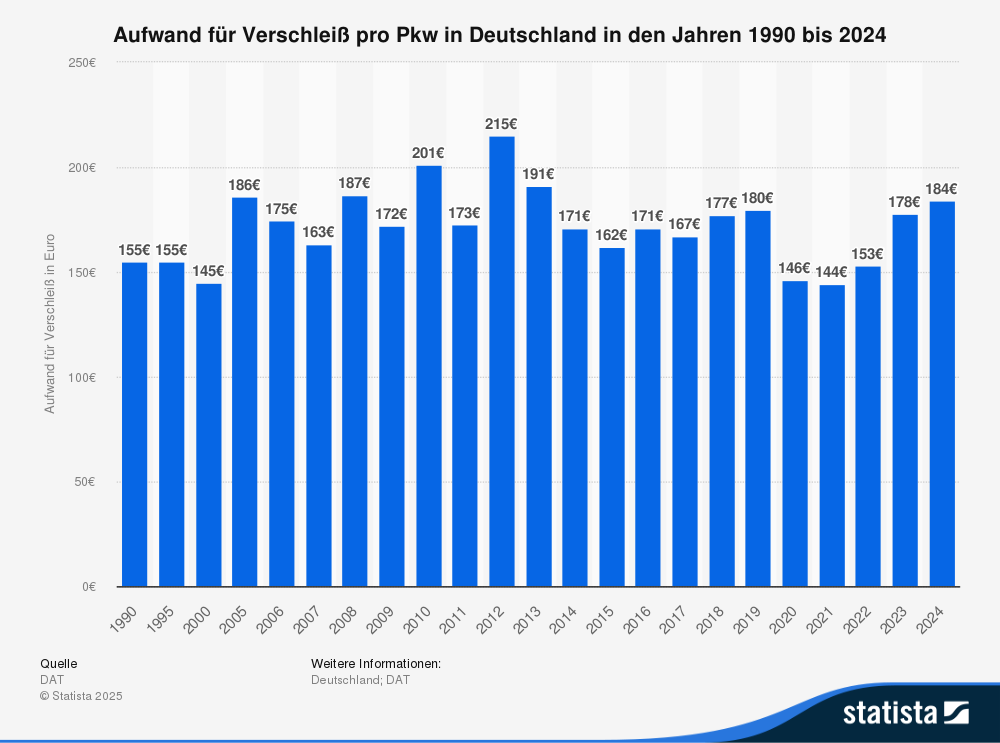
\includegraphics[width=0.75\linewidth]{images//wettbewerb/statistic_id39416_aufwand-fuer-verschleiss-pro-pkw-in-deutschland-2024.png}
    \caption{Durchschnittlicher Aufwand für Verschleiß pro Pkw in Deutschland im Jahr 1990 bis 2024 \citep{zdk2025verschleiss}}
    \label{fig:verschleiss}
\end{figure}

Ein Blick auf die Entwicklung der Verschleißkosten pro Pkw (Abb. \ref{fig:verschleiss}) in Deutschland zwischen 1990 und 2024 verdeutlicht, dass sich diese im Zeitverlauf nur geringfügig verändert haben. Nach einem kontinuierlichen Anstieg bis zum Jahr 2012, in dem mit 215 Euro ein Höhepunkt erreicht wurde, sind die Kosten in den darauffolgenden Jahren wieder gesunken und pendeln sich aktuell bei etwa 150 bis 180 Euro ein. Dies deutet darauf hin, dass Verschleißteile durch technologische Fortschritte langlebiger geworden sind und ein intensiver Wettbewerb im Ersatzteilmarkt für stabile Preise sorgt. Für Werkstätten bedeutet dies, dass das klassische Ersatzteilgeschäft nur begrenztes Wachstumspotenzial bietet und nicht mehr als Haupttreiber für Umsatzsteigerungen betrachtet werden kann. \citep[vgl.][]{zdk2025verschleiss}

\begin{figure}[h!]
    \centering
    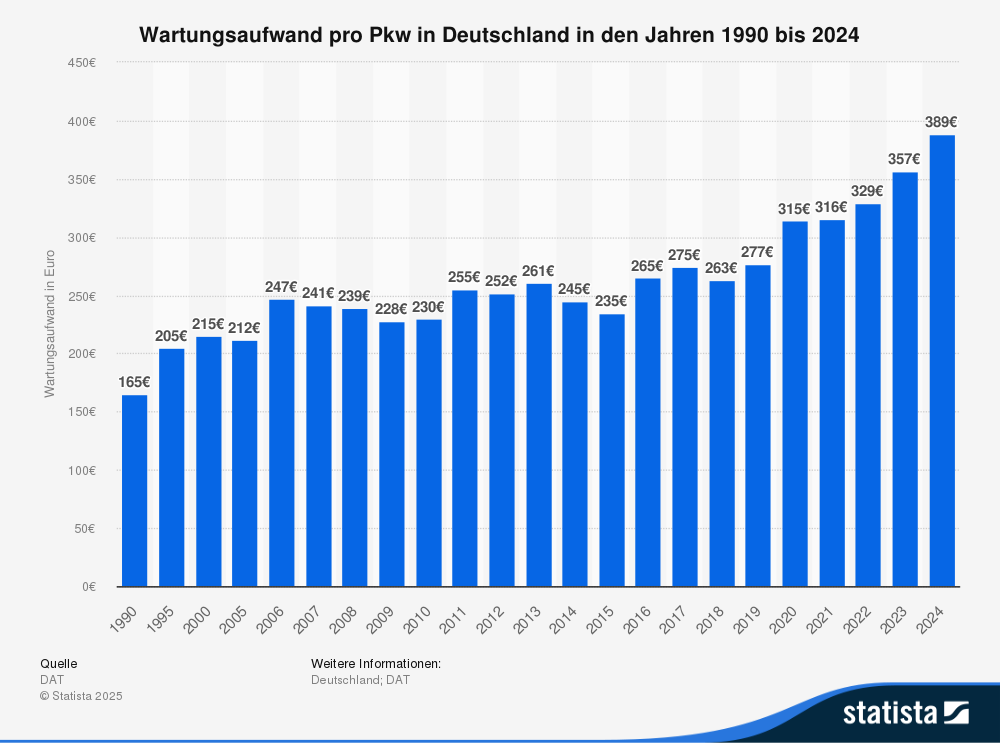
\includegraphics[width=0.75\linewidth]{images//wettbewerb/statistic_id39415_wartungsaufwand-pro-pkw-in-deutschland-bis-2024.png}
    \caption{Durchschnittlicher Aufwand für Wartung pro Pkw in Deutschland im Jahr 1990 bis 2024 \citep{zdk2025wartungsaufwand}}
    \label{fig:aufwand}
\end{figure}

Deutlich dynamischer stellt sich hingegen die Entwicklung der Wartungskosten dar (Abb. \ref{fig:aufwand}). Während diese 1990 noch bei 165 Euro pro Fahrzeug lagen, stiegen sie bis 2024 auf knapp 390 Euro an. Besonders in den letzten Jahren hat sich die Kurve stark nach oben entwickelt. Ursache hierfür ist die wachsende technische Komplexität moderner Fahrzeuge, die zunehmend mit elektronischen Steuerungen, Softwarelösungen und Fahrerassistenzsystemen ausgestattet sind. Für Werkstätten entsteht hieraus ein erhebliches Umsatzpotenzial, gleichzeitig jedoch auch ein wachsender Kostendruck auf die Kunden, die mit höheren Rechnungsbeträgen konfrontiert werden. Daraus resultiert eine zunehmende Preissensibilität, die den Wettbewerb zwischen Werkstätten verschärft. \citep[vgl.][]{zdk2025wartungsaufwand}

\begin{figure}[h!]
    \centering
    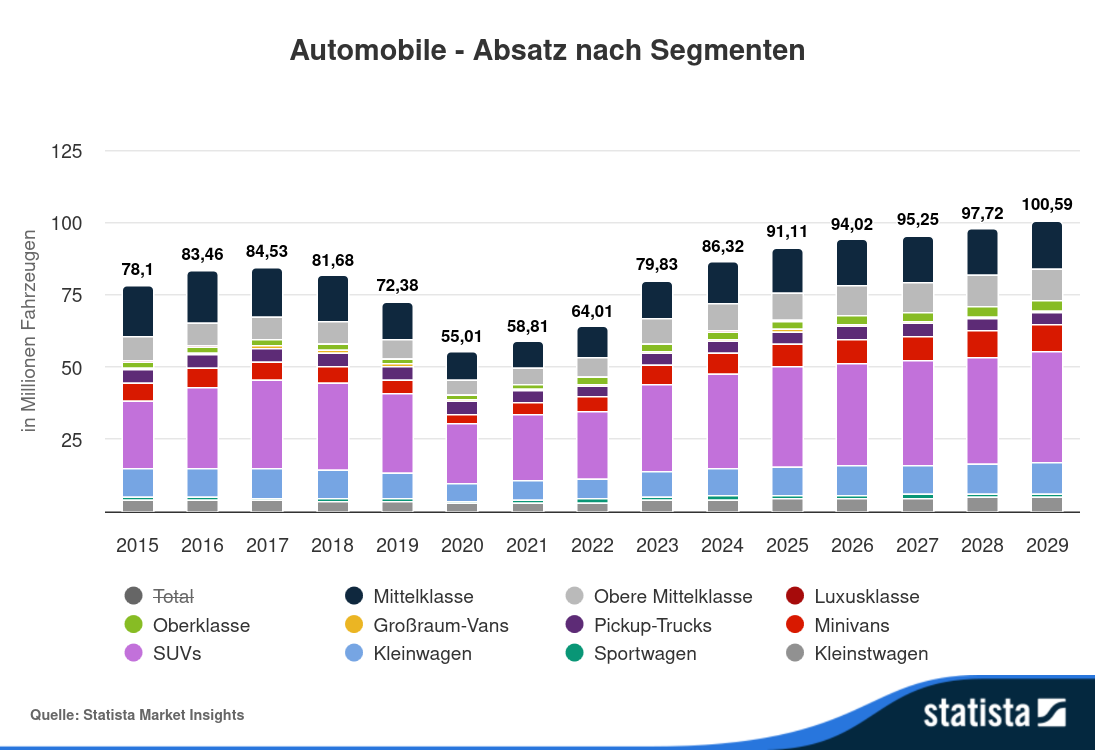
\includegraphics[width=0.75\linewidth]{images//wettbewerb/Statista-Market-Insights--Automobile-Weltweit--Absatz-nach-Segmenten.png}
    \caption{Weltweiter Absatz von Automobilen nach Segmenten im Zeitraum 2015 bis 2029 \citep[][]{statista2025automobile}}
    \label{fig:placeholder}
\end{figure}

Parallel dazu verändert sich der Automobilmarkt selbst. Die weltweiten Absatzzahlen zeigen, dass die Nachfrage nach Fahrzeugen seit dem pandemiebedingten Einbruch im Jahr 2020 wieder deutlich steigt und bis 2029 die Marke von 100 Millionen verkauften Fahrzeugen überschreiten dürfte. Auffällig ist die wachsende Bedeutung von SUVs und Fahrzeugen der Mittel- und Oberklasse. Diese Fahrzeuge sind häufig wartungsintensiver und erfordern spezialisierte Diagnosetechnik sowie regelmäßige Softwareupdates. Für Werkstätten bedeutet dies einerseits die Chance auf zusätzliche Wartungsumsätze, andererseits aber auch die Notwendigkeit, kontinuierlich in moderne Diagnosegeräte und in die Weiterbildung der Mitarbeiter zu investieren. Der Wettbewerb wird sich daher nicht mehr allein über Preis und Servicequalität entscheiden, sondern zunehmend auch über technologische Kompetenz und Spezialisierung. \citep[vgl.][]{statista2025automobile}

\begin{figure}[h!]
    \centering
    \begin{subfigure}[t]{0.7\linewidth}
        \centering
        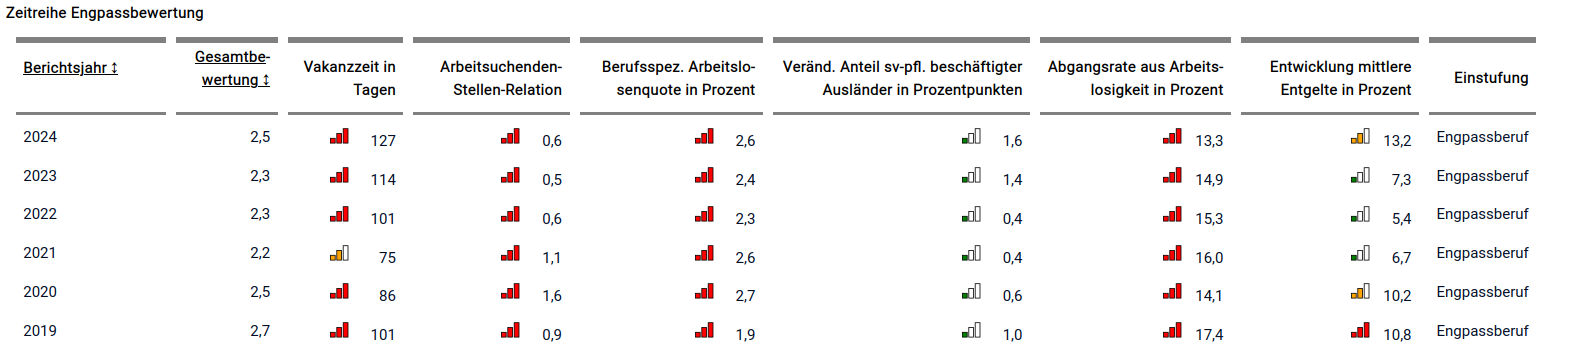
\includegraphics[width=\linewidth]{images/wettbewerb/fach_engpass.png}
        \caption{Entwicklung des Fachkräfteengpasses}
        \label{fig:fach_engpass}
    \end{subfigure}
    \hfill
    \begin{subfigure}[t]{0.26\linewidth}
        \centering
        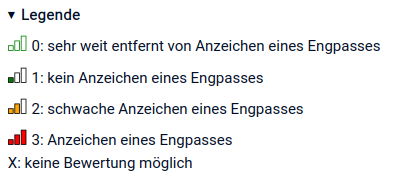
\includegraphics[width=\linewidth]{images/wettbewerb/legnde_fach.png}
        \caption{Legende Fachkräfteengpasses}
        \label{fig:legende_fach}
    \end{subfigure}
    \caption{Fachkräfteengpass in den Berufen der Mechatronik (2611) in Deutschland \citep[][]{ba2025engpassanalyse2611}}
    \label{fig:nebeneinander}
\end{figure}


Neben diesen marktwirtschaftlichen Faktoren stellt der Fachkräftemangel eine der größten Herausforderungen dar. Die Engpassbewertung für den Beruf des Kfz-Mechatronikers zeigt, dass dieser seit Jahren als Engpassberuf gilt. Die durchschnittliche Vakanzzeit bei offenen Stellen beträgt inzwischen 127 Tage, während die Relation von Arbeitsuchenden zu gemeldeten Stellen mit 0,6 sehr niedrig ist. Dies bedeutet, dass es erheblich mehr offene Stellen als verfügbare Fachkräfte gibt. Trotz steigender Bedeutung des Berufs, bedingt durch die zunehmende Komplexität der Fahrzeuge, gelingt es der Branche nicht, ausreichend Nachwuchs zu gewinnen. Für Werkstätten entsteht hier ein doppelter Druck: Einerseits wächst die technische Anforderung an die Arbeit, andererseits fehlen die qualifizierten Arbeitskräfte, um diese Nachfrage zu decken. \citep[vgl.][]{ba2025engpassanalyse2611}
\newline\newline
Zusammenfassend lässt sich feststellen, dass die Kfz-Werkstattbranche in den kommenden Jahren mit mehreren parallelen Entwicklungen umgehen muss. Während Verschleißkosten stagnieren, eröffnen steigende Wartungskosten zusätzliche Umsatzpotenziale. Gleichzeitig erfordern die Veränderungen im Automobilmarkt, insbesondere die wachsende Nachfrage nach SUVs und technisch anspruchsvolleren Fahrzeugen, höhere Investitionen in Technik und Know-how. Hinzu kommt der Fachkräftemangel, der die Wettbewerbsfähigkeit vieler Betriebe unmittelbar bedroht. Werkstätten, die langfristig erfolgreich sein wollen, müssen daher einerseits technologische Innovationsfähigkeit entwickeln und andererseits attraktive Arbeitsbedingungen schaffen, um Fachkräfte zu gewinnen und zu binden. Nur so lässt sich der steigende Kostendruck mit einer nachhaltigen Wettbewerbsstrategie ausgleichen. Gerade an dieser Stelle setzt KARL Diagnostics an. Das System unterstützt Werkstätten dabei, den steigenden technischen Anforderungen gerecht zu werden, ohne dass hierfür unverhältnismäßig hohe Investitionen in Spezialwissen oder zusätzliche Fachkräfte notwendig sind. Durch die Kombination aus automatisierter Fehleranalyse, KI-gestützter Ursachenfindung und transparenten Handlungsempfehlungen können auch weniger erfahrene Mitarbeiter komplexe Diagnosen zuverlässig durchführen. Auf diese Weise wird der Fachkräftemangel teilweise kompensiert, da die Abhängigkeit von hochspezialisierten Technikern reduziert wird. Gleichzeitig profitieren Betriebe von einer höheren Effizienz, geringeren Fehlerraten und einer schnelleren Abwicklung von Reparaturaufträgen. Ein weiterer Vorteil liegt in der kontinuierlichen Erweiterung des Systems durch Herstellerinformationen und Erfahrungsberichte aus der Praxis. So bleiben Werkstätten technologisch auf dem neuesten Stand, ohne permanent in teure Weiterbildungen oder proprietäre Diagnosesysteme investieren zu müssen. KARL Diagnostics fungiert damit nicht nur als technisches Werkzeug, sondern als strategischer Enabler, der den Spagat zwischen Kostendruck, Fachkräftemangel und steigender Komplexität moderner Fahrzeuge erleichtert und die Wettbewerbsfähigkeit langfristig sichert.

\subsection{Wettbewerbsumfeld und potentielle Konkurrenten}
Der Wettbewerb in der Kfz-Diagnose- und Werkstattsoftwarebranche ist stark fragmentiert. Auf der einen Seite stehen große, etablierte Anbieter von Diagnosetechnik wie Bosch, Hella Gutmann oder Delphi Technologies, die Werkstätten mit umfangreichen, oft herstellerspezifischen Lösungen versorgen. Diese Systeme sind leistungsfähig, erfordern jedoch häufig hohe Investitionen in Lizenzen, Hardware und regelmäßige Updates. Zudem sind sie meist komplex in der Anwendung, was die Abhängigkeit von hochqualifizierten Fachkräften verstärkt. \citep[vgl.][]{delphi2025dsdiagnosesoftware,bosch2025diagnosegeraete,hellagutmann2025diagnoseloesungen}
\newline\newline
Daneben existiert eine Vielzahl kleinerer Anbieter, die sich auf Nischenlösungen spezialisiert haben, etwa für bestimmte Fahrzeugmarken oder Teilbereiche wie Motorsteuerung, Klimasysteme oder elektrische Komponenten. Diese Tools sind oftmals günstiger, decken jedoch nur eingeschränkte Anwendungsfälle ab und bieten nicht die breite Abdeckung, die freie Werkstätten für den Alltag benötigen. Ein weiterer Wettbewerbsfaktor sind die herstellereigenen Diagnosesysteme, die von Fahrzeugproduzenten zunehmend auch für unabhängige Werkstätten zugänglich gemacht werden. Diese Systeme sind in Bezug auf Aktualität und Funktionsumfang häufig überlegen, binden die Werkstätten jedoch stärker an die jeweiligen Hersteller und schränken ihre Flexibilität im Mehrmarkengeschäft ein.
\newline\newline
Im Vergleich dazu positioniert sich KARL Diagnostics als herstellerunabhängige, \ac{KI}-gestützte Lösung, die den Spagat zwischen Funktionsbreite, Kostenkontrolle und Benutzerfreundlichkeit ermöglicht. Während traditionelle Systeme stark auf Expertenwissen angewiesen sind, verfolgt KARL einen Ansatz, der gerade weniger erfahrenen Mitarbeitern eine sichere und effiziente Fehleranalyse erlaubt. Damit unterscheidet sich KARL sowohl von den etablierten Komplettlösungen mit hohen Investitionshürden als auch von den spezialisierten Nischenprodukten, die oft nur begrenzte Einsatzmöglichkeiten bieten.




